\clearpage
% Set chapter counter to 2 and reset section counter
\setcounter{chapter}{2}
\setcounter{section}{0}

% Add the chapter to table of contents
\addcontentsline{toc}{chapter}{\numberline{2}Rethinking Democratization: Beyond Access to Preservation}

% Set up page style for this chapter (assuming fancyhdr is loaded in preamble)
\pagestyle{fancy}
\fancyhf{} % Clear all header and footer fields
\fancyhead[L]{\footnotesize\textit{Ars Post Faber: Digital Fabrication Democratization Through Embodied Knowledge Preservation}}
\fancyfoot[C]{\thepage} % Page number in footer center
\renewcommand{\headrulewidth}{0pt}
\renewcommand{\footrulewidth}{0pt}

% Custom chapter title to match abstract formatting
\noindent
{\Large\textbf{Chapter 2: Rethinking Democratization: Beyond Access to Preservation}}
\vspace{0.3cm}
\hrule
\vspace{0.8cm}
\label{ch:democratization}

% Set no paragraph indentation
\setlength{\parindent}{0pt}

The historical trajectory examined in Chapter 1 has showed how creative agency has been systematically redistributed from unified practice to contemporary digital workflows. This analysis raises the question: if digital fabrication technologies possess unprecedented capabilities for material manipulation and geometric exploration, why do they continue to perpetuate the same distributed agency frameworks that eliminated adaptive authority? The answer lies in how the "democratization" itself has been conceptualized within digital fabrication discourse.

\vspace{0.5cm}

Rather than addressing the organizational structures that fragment creative agency, contemporary digital fabrication has pursued democratization primarily through expanded access to scaled-down industrial tools. This chapter will examine how this access-centered approach, while achieving remarkable quantitative success, fails to address the deeper structural issues identified in the historical analysis. By tracing the evolution from access-based democratization toward preservation-centered approaches, this chapter will try to pursue a reconceptualization of what democratic making might mean in digital contexts.

\section{The Access Paradigm and Its Achievements}

This access-centered understanding of democratization has become the dominant paradigm within contemporary digital fabrication discourse. Neil Gershenfeld's\footnote{Neil Gershenfeld is a physicist at MIT who's the director of the Center for Bits and Atoms (CBA) and pioneered the global FabLab movement. His work focuses on the intersection of physical and digital systems, advocating for "personal fabrication" as a means to democratize access to manufacturing capabilities.} foundational vision for FabLabs\footnote{FabLabs (Fabrication Laboratories) are digital fabrication workshops that provide public access to tools for invention, prototyping and local production. Originally conceived at MIT's Center for Bits and Atoms, FabLabs follow a global charter emphasizing open access, education, and local innovation while connecting to a worldwide network of collaborative spaces.} promised "personal fabrication" enabling "almost anyone to make almost anything" \citep{gershenfeld2007}, positioning digital fabrication as the natural evolution of personal computing—bringing the same accessibility that desktop computers brought to information processing into the realm of physical manufacturing. This vision emphasized scaling down industrial production capabilities to individual users, making sophisticated fabrication tools available in community workshops and educational institutions.

\vspace{0.5cm}

\begin{figure}[h]
\centering
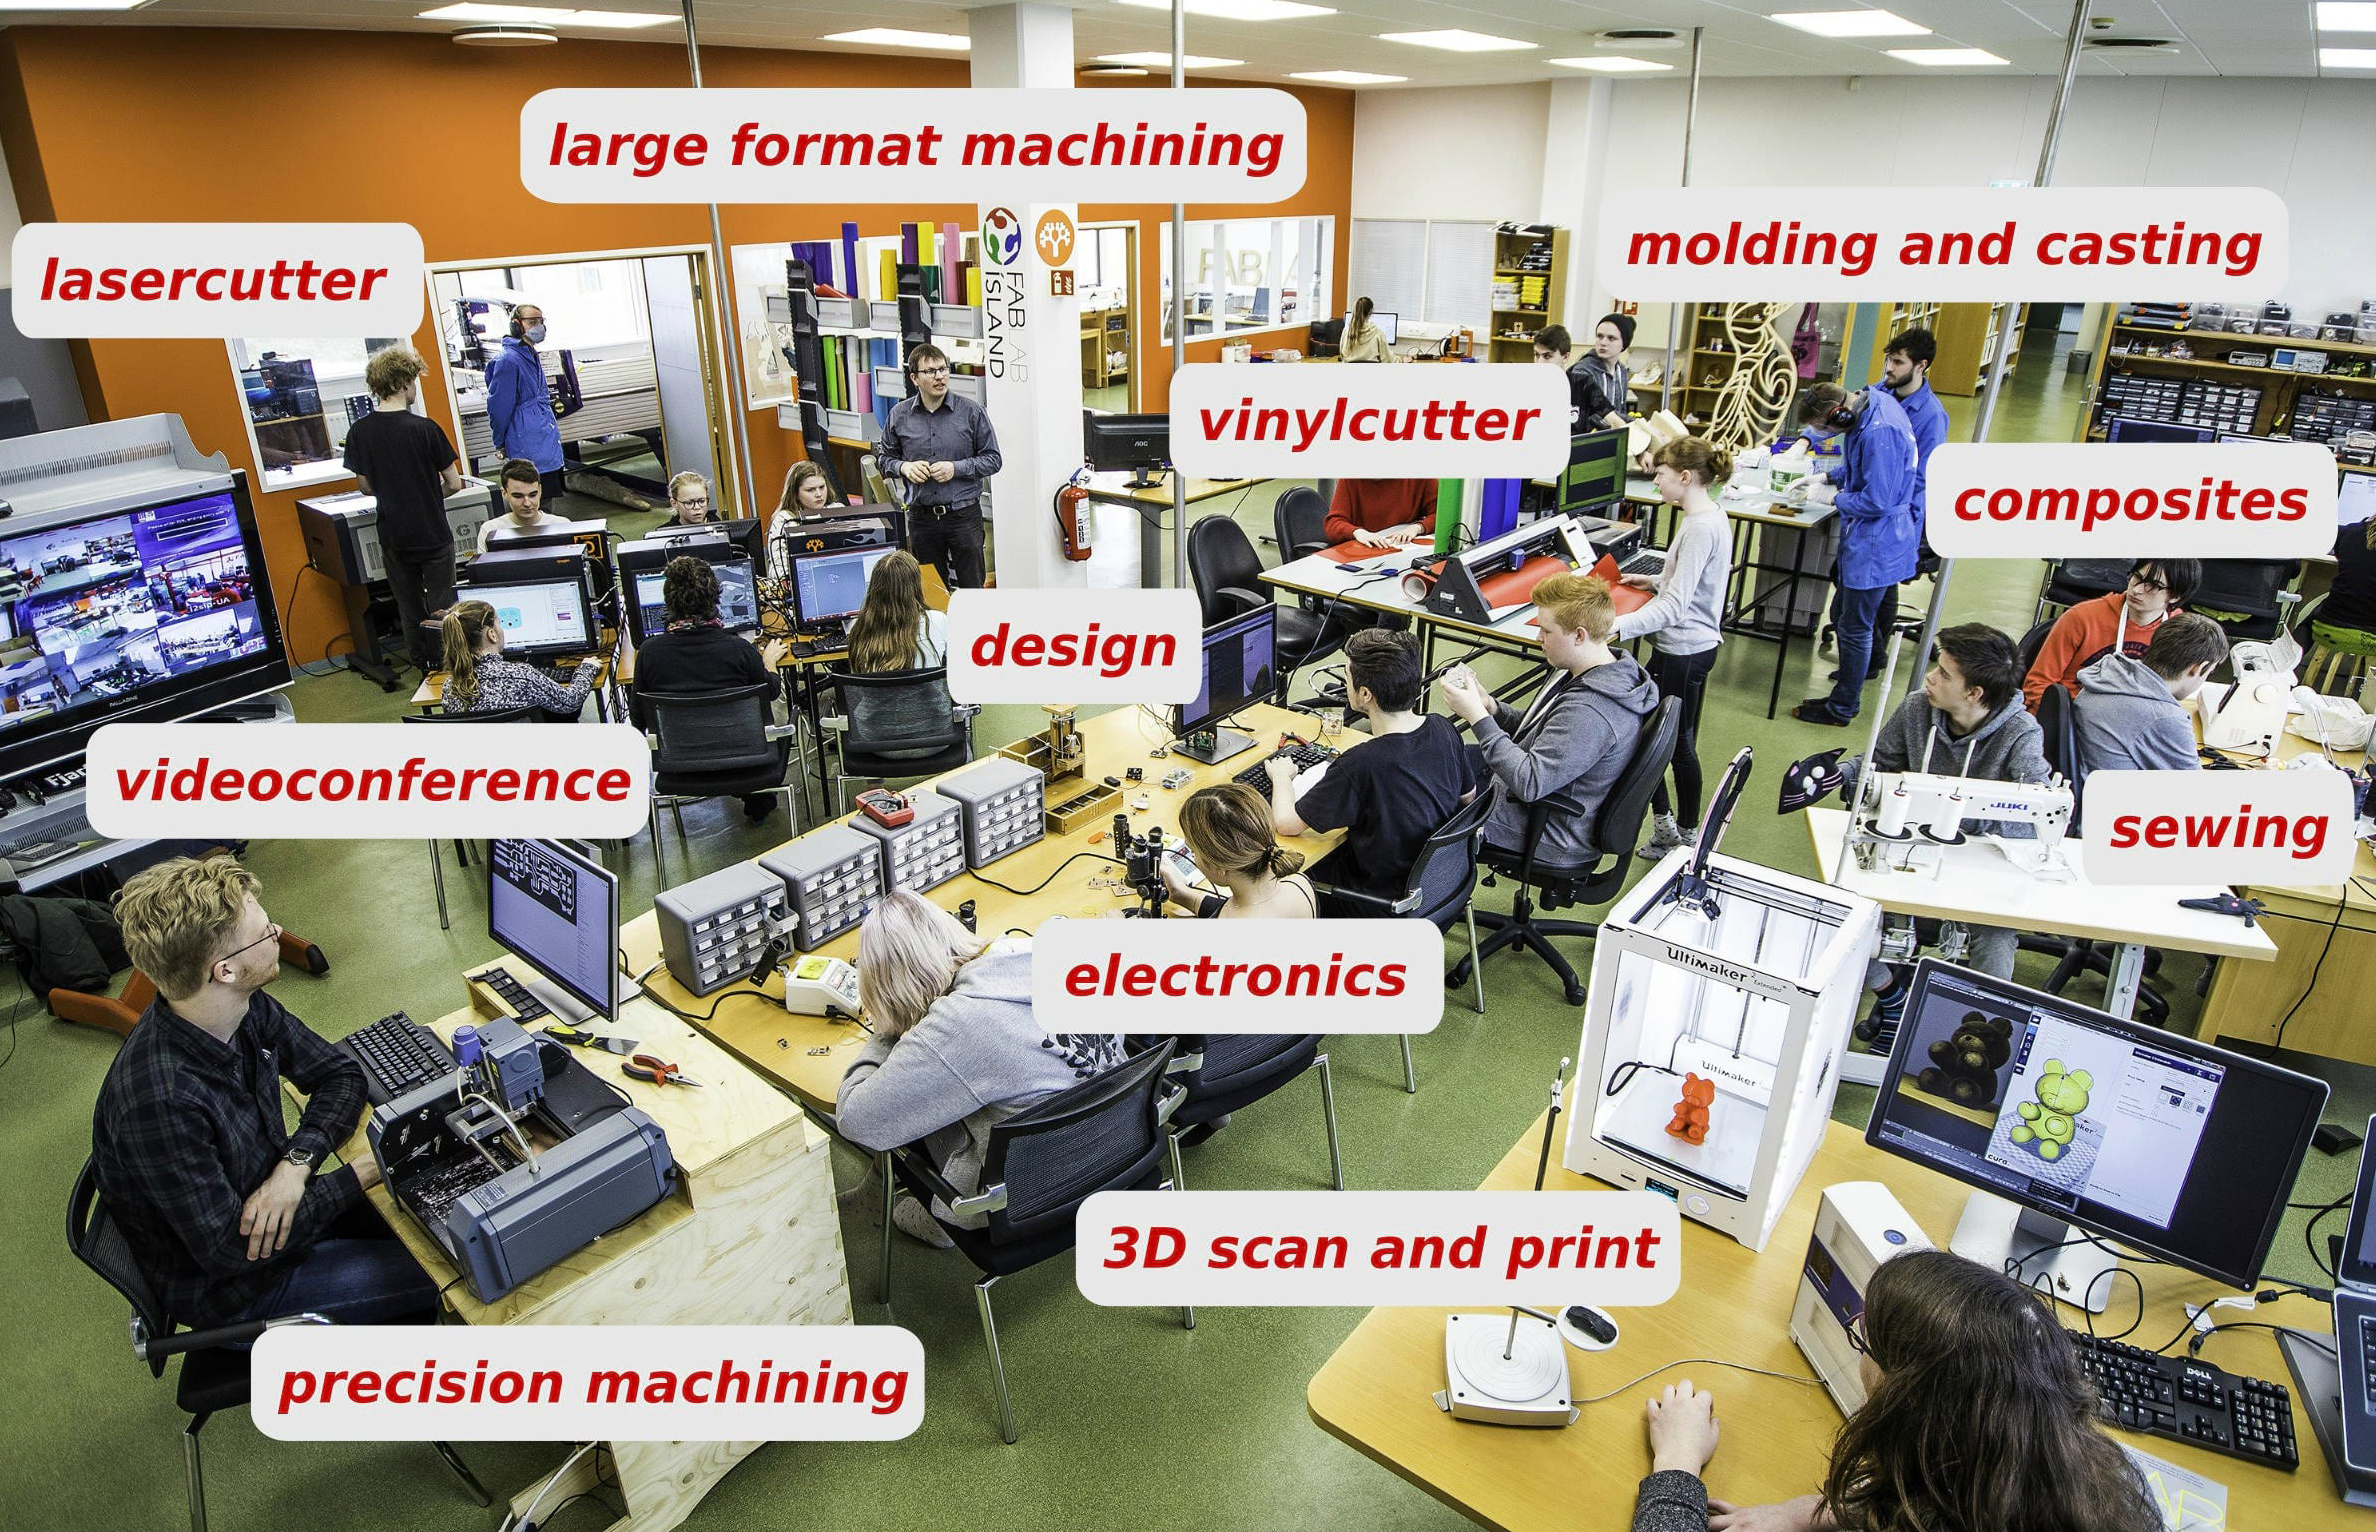
\includegraphics[width=1\textwidth]{figures/chapter2/fablab_tools.jpg}
\caption{Tools in a Fab Lab. Source: Fab Foundation, 2024}
\label{fig:fablab_tools}
\end{figure}

Building on this foundation, the broader maker movement, as articulated by Mark Hatch, advocated for "radically democratizing access to the tools of innovation" \citep{hatch2013}, framing making as both a form of personal empowerment and economic opportunity. Hatch's manifesto positioned the maker movement as a response to mass production's alienation, promising that widespread access to fabrication tools would restore individual agency in production while fostering innovation and entrepreneurship at the grassroots level.

\vspace{0.5cm}

This approach has achieved remarkable quantitative success: from fewer than 50 FabLabs worldwide in 2009 to over 2,000 by 2023 \citep{fabfoundation2024}, there's been an unprecedented expansion of access to sophisticated production capabilities.

\begin{figure}[h]
\centering
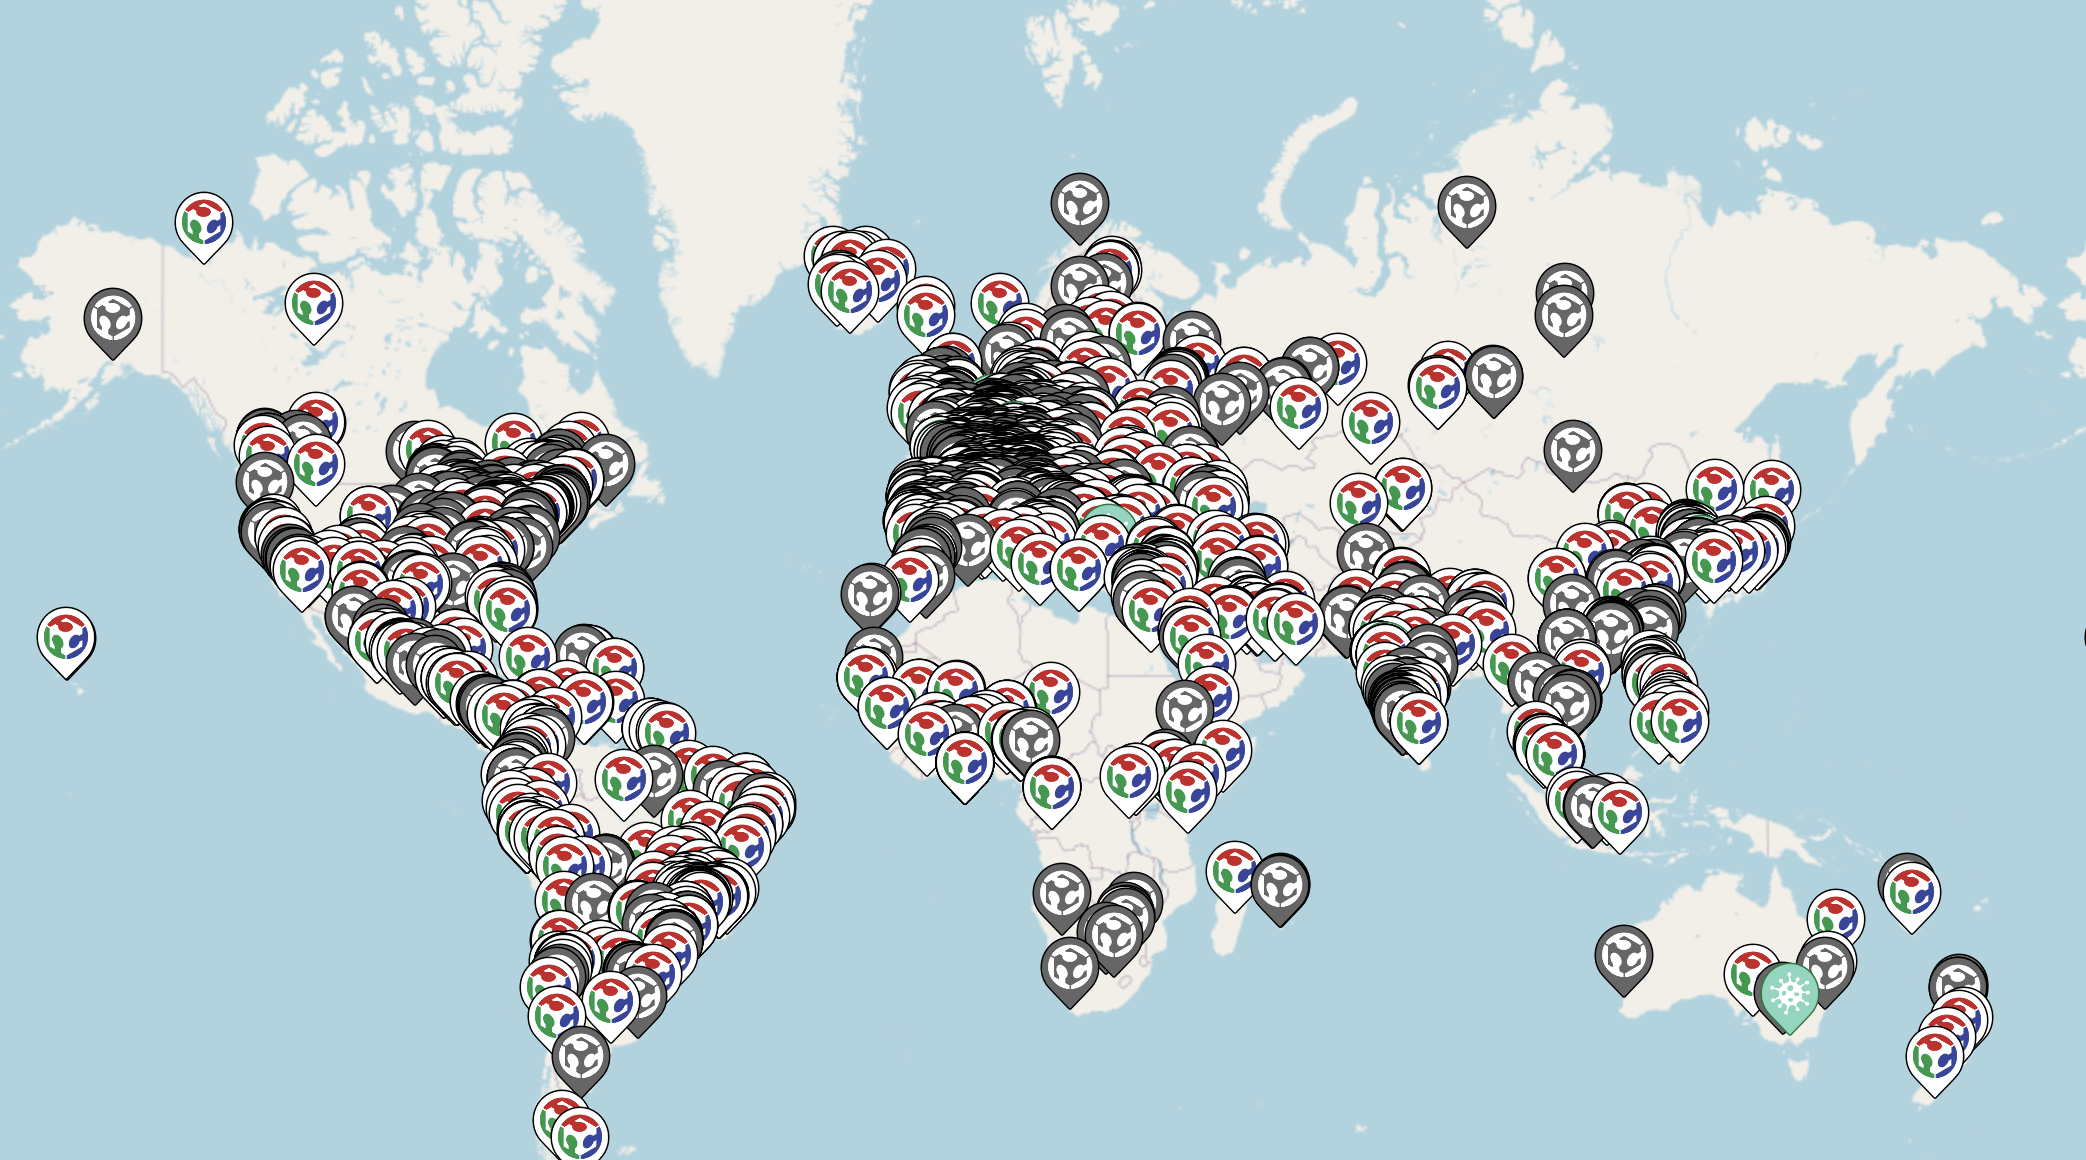
\includegraphics[width=1\textwidth]{figures/chapter2/fablabsmap.png}
\caption{Global distribution of FabLabs. Map showing the locations of FabLabs around the world. Source: Fab Foundation, 2024}
\label{fig:fablabs_map}
\end{figure}

This democratization of digital fabrication extends beyond physical tools to software infrastructures. Open-source\footnote{Open-source software is developed with publicly accessible source code, allowing users to modify, improve the software and in some cases even distribute it.} and free CAD alternatives like FreeCAD\footnote{FreeCAD is a parametric 3D CAD modeler designed for mechanical engineering and product design, available as free and open-source software.}, Blender\footnote{Blender is an Open-Source 3D creation suite supporting modeling, animation, rendering, and video editing, mainly used for animation but increasingly used for CAD applications.} or TinkerCAD\footnote{TinkerCAD is a web-based 3D design application developed by Autodesk, designed for beginners with simplified modeling tools and browser-based accessibility.} combined with educational programs to know how to use the tools, have reduced barriers to digital design literacy. Contemporary maker spaces enable individual access to CNC machines\footnote{Computer Numerical Control (CNC) machines use computer-controlled cutting tools to precisely shape materials like wood, metal, and plastic from digital designs.}, 3D printers\footnote{3D printers create physical objects by depositing material layer by layer based on digital 3D models, enabling rapid prototyping and small-scale production.}, and laser cutters\footnote{Laser cutters use focused laser beams to cut or engrave materials with high precision, commonly used for creating flat parts from sheet materials like wood, acrylic, and metal.} for modest fees (sometimes even for free), genuinely transforming the economic conditions of making.

\vspace{0.5cm}

Yet this access-focused paradigm highlights certain limitations when examined against historical precedents of successful democratization movements. The expansion of who can use fabrication tools does not address how those tools structure agency within making processes. As Tanenbaum et al. observe, maker practices still depend heavily on existing industrial infrastructure and face challenges "when it comes to scaling up production and distribution" \citep{tanenbaum2013}.

\section{The Preservation Problem: What Access Cannot Address}

While the quantitative expansion of fabrication access represents genuine progress, it reveals limitations in how democratization has been conceptualized. What contemporary digital fabrication lacks is what this research identifies as a preservation problem: the loss of tacit knowledge and embodied practices that characterize skilled making. This goes beyond the historical fragmentation patterns analyzed in Chapter 1 to encompass how knowledge itself is transmitted, maintained, and evolved within making communities.

\vspace{0.5cm}

Richard Sennett's analysis of craftsmanship emphasizes that "the desire to do something well for its own sake" \citep{sennet2009} requires forms of embodied learning that resist systematic codification. Unlike explicit knowledge that can be documented in manuals or encoded in software, tacit knowledge emerges through sustained engagement with materials, tools, and techniques.

\vspace{0.5cm}

Contemporary digital fabrication workflows eliminate opportunities for this knowledge transmission. While FabLabs and maker spaces provide access to sophisticated tools, they typically operate through standardized tutorials and predetermined project sequences that prioritize rapid skill acquisition over deep material understanding. The emphasis on "democratizing" access often translates into simplifying workflows to reduce learning curves, eliminating the complex, time-intensive processes through which tacit knowledge traditionally develops.

\vspace{0.5cm}

This preservation problem manifests through persistent organizational structures that extend beyond individual tool use. Despite the collaborative and educational dimensions of maker spaces, the workflow architecture maintains the distributed agency pattern traced in Chapter 1. Creative decisions remain concentrated in separate design phases, while material execution follows predetermined procedures that eliminate opportunities for the responsive adaptation. The result is a democratization that provides access to tools without preserving the knowledge systems that enable those tools to support genuine creative agency.

\vspace{0.5cm}

The insight that emerges from this analysis is that democratization cannot be achieved through access alone, it requires organizational innovation that preserves the continuity of creative decision-making throughout the making process. This shifts focus from who can use fabrication tools to how those tools can be structured to maintain what was identified in Chapter 1 as unified agency. 

\section{Redefining Democratization: Process Over Access}

Through the analysis of the preservation problem it's possible to raise the question about how "democratization" has been conceptualized within digital fabrication discourse. While the term implies expanding democratic participation, current approaches, as mentioned, focus primarily on access expansion rather than examining what democratic participation actually requires. Before proposing alternative models for fabrication democratization, it becomes necessary to question what "democracy" itself demands and how those requirements might apply to making contexts.

\vspace{0.5cm}

The analysis of different precedents and patterns suggest that democratization movements across multiple domains initially focus on access expansion before recognizing deeper structural challenges. Political democratization, educational reform, and cultural preservation movements all showcase patterns that would align with it: early phases emphasize expanding participation within existing systems, while later phases require fundamental transformation of the systems themselves. For instance, political democratization initially focused on expanding voting rights, but later required systematic changes like proportional representation systems such as the D'Hondt method\footnote{The D'Hondt method is a proportional representation electoral system that allocates seats based on vote share, developed to ensure more democratic representation beyond simple majority voting.} to ensure genuine democratic representation rather than mere voting access. Similarly, educational democratization moved beyond simply expanding school enrollment to developing pedagogical approaches that understand and accommodate diversity in the classroom, adapting curricula to different learning styles and cultural backgrounds rather than imposing standardized approaches. These precedents suggest that fabrication democratization may be encountering similar limitations inherent to access-based approaches.

\vspace{0.5cm} 

Rather than assuming that broader tool access automatically produces democratic participation, the following analysis will examine what democracy actually requires and how those requirements might inform alternative approaches to fabrication democratization. By analyzing democratic theory alongside cross-cultural preservation practices, this chapter will attempt to develop frameworks for distinguishing between superficial access and substantive democratic participation in production processes.

\section{Deconstructing "Democratization": What Democracy Actually Requires}

The theoretical framework established requires a deeper examination of the term "democratization" itself and its specific application to fabrication contexts. While democratic theory provides extensive analysis of political participation, its principles have been applied to fabrication with insufficient critical examination of what democratic participation might actually require within making processes. The word "democracy" derives from the Greek {\greekfont δημοκρατία} (demokratia) demos (people) + kratos (power/rule), meaning rule by the people. This etymology suggests that democratization involves the distribution of ruling authority rather than expanded access to predetermined systems, a distinction with big implications for how fabrication democratization should be conceptualized.

\vspace{0.5cm}

Political democracy, at its core, requires the distribution of decision-making authority among participants rather than merely access to predetermined decision-making processes. As Robert Dahl's\footnote{Robert A. Dahl (1915--2014) was an American political theorist whose work on democratic theory, shaped contemporary understanding of democratic systems and citizen engagement.} foundational analysis demonstrates, democratic systems must provide "effective participation" \citep{coglianese1990} where citizens have "basic political rights and liberties, such as free expression, and allows persons to live under laws of their own choosing" \citep{coglianese1990}, and enlightened understanding enabling informed choice among alternatives. Crucially, democracy requires what Dahl terms "final control over the agenda" \citep{mayhew2017}, the authority to determine not just outcomes within predetermined options, but the capacity to define what questions get asked and how they are framed. Distinguishing genuine democratic participation from consultative processes that solicit input within predetermined parameters while concentrating agenda-setting authority elsewhere.

\vspace{0.5cm}

Applied to fabrication contexts, this analysis reveals that current maker spaces, despite their collaborative ethos, preserve a fabrication autocracy, a system that concentrates creative authority in separate design phases while relegating material execution to predetermined procedures that eliminate participant agency. Genuine fabrication democratization would require the distribution of creative decision-making authority throughout making processes, enabling makers to exercise "final control over the agenda" not just in initial design specification, but in determining how fabrication workflows themselves operate and evolve in response to material conditions and emergent discoveries.

\section{The Representation Problem in Fabrication Democracy}

Having established that genuine democratization requires the distribution of decision-making authority rather than mere access expansion, it becomes necessary to examine how such authority might be structured within fabrication contexts. Political democracy usually confronts the challenge of representation: how to enable large-scale collective decision-making while preserving individual agency? This requires sophisticated institutional frameworks, electoral systems, deliberative processes, and constitutional protections that mediate between individual preferences and collective outcomes without eliminating personal autonomy.

\vspace{0.5cm}

Fabrication democratization faces analogous representational challenges: how to enable collective access to sophisticated manufacturing capabilities while preserving individual makers' authority to determine their own creative processes? Yet current digital fabrication has developed no equivalent to democratic political institutions. Instead, it has adopted  a technocratic representation, expert-designed software interfaces and standardized file formats that mediate between human intention and material execution while eliminating opportunities for maker input beyond initial design specification.

\vspace{0.5cm}

This technocratic approach mirrors Joseph Schumpeter's\footnote{Joseph Schumpeter (1883-1950) was an Austrian economist and politic who developed influential theories about capitalism and democratic systems.} theory of democracy as "competitive leadership" \citep{schumpeter1950}, a system that preserves formal democratic procedures while concentrating substantive decision-making authority within expert institutions. Just as this limited democracy enables citizen participation within predetermined choices while eliminating popular control over the agenda setting, just as current fabrication democratization enables maker participation within predetermined expert designed workflow structures while eliminating authority over how those structures have to be operated.




